% energy_change.png: the clusters that change when two sites exchange their atoms. Make it in this folder with, for any scratch folder T:
%   pdflatex -output-directory=T fig_energy_change.tex
%   python3 pdf_to_png.py T/fig_energy_change.pdf ../energy_change.png
\documentclass[11pt,tikz,border=1.5pt]{standalone}
% Shared preamble of all figures. Every fig_*.tex is compiled on its own, see the comment at its top; the fonts are those of the matplotlib
% style xzc_sans (amsmath, amssymb, amsfonts, sfmath), so that line drawings and data plots look the same.
\usepackage{amsmath,amssymb,amsfonts}
\usepackage{sfmath}
\renewcommand{\familydefault}{\sfdefault}
\usepackage{graphicx}
\usetikzlibrary{arrows.meta,calc,positioning,decorations.pathreplacing,backgrounds,shapes.geometric}
% species: Al gray, Mg orange, Zn blue; red marks the vacancy and the jumping atom
\definecolor{cAl}{HTML}{B8BCC2}
\definecolor{cMg}{HTML}{E08A2E}
\definecolor{cZn}{HTML}{3F78B5}
\definecolor{cOne}{HTML}{C8423B}
\definecolor{cTwo}{HTML}{3F78B5}
\definecolor{cThree}{HTML}{3E9B5C}
\definecolor{cFour}{HTML}{E0A21B}
\definecolor{cGray}{HTML}{7E858F}
\definecolor{cDark}{HTML}{2B2B2B}
\newcommand{\panel}[1]{\textbf{(#1)}}
\newcommand{\DM}{D_{\mathrm{MEP}}}
\newcommand{\KI}{K_{\mathrm{I}}}
\newcommand{\KF}{K_{\mathrm{F}}}
\newcommand{\dE}{\Delta E}
\newcommand{\Ea}{\Delta E_{\mathrm{a}}}
\newcommand{\ea}{\Delta e_{\mathrm{a}}}
\newcommand{\Ebind}{E_{\mathrm{bind}}^{\mathrm{site}}}
% a ball with a soft highlight, like the rendered spheres
\makeatletter
\pgfdeclareradialshading[tikz@ball]{softball}{\pgfpoint{-9bp}{9bp}}{%
  color(0bp)=(tikz@ball!22!white); color(6bp)=(tikz@ball!62!white); color(13bp)=(tikz@ball!96!white);
  color(20bp)=(tikz@ball!92!black); color(27bp)=(tikz@ball!74!black); color(50bp)=(tikz@ball!55!black)}
\makeatother
\tikzset{
  every picture/.append style={line cap=round, line join=round},
  every node/.append style={font=\small},
  img/.style={inner sep=0pt, anchor=south west},
  lab/.style={font=\normalsize, inner sep=1pt, anchor=north west},
  above lab/.style={font=\normalsize, inner sep=1pt, anchor=south west},
  capt/.style={align=center, anchor=north},
  atom/.style={circle, ball color=#1, shading=softball, minimum size=12pt, inner sep=0pt},
  atom/.default=cAl,
  vac/.style={circle, draw=cOne, line width=1.1pt, fill=white, minimum size=11.5pt, inner sep=0pt},
  arr/.style={-{Stealth[length=5pt]}, line width=0.8pt},
  dbl/.style={{Stealth[length=4pt]}-{Stealth[length=4pt]}, line width=0.8pt},
  jump/.style={arr, cOne, line width=1.2pt},
  block/.style={-{Triangle[length=8pt, width=13pt]}, line width=5pt, cTwo!38},
  cell axis/.style={-{Triangle[length=6pt, width=5.5pt]}, line width=1.2pt, black},
  dir/.style={fill=white, fill opacity=0.75, text opacity=1, font=\footnotesize, inner sep=1.5pt},
}
\graphicspath{{img/}}
% data plots are included at one scale: \plot{name}{x}{y}{file}
\newcommand{\plotscale}{0.6}
\newcommand{\plot}[4]{\node[img] (#1) at (#2,#3) {\includegraphics[scale=\plotscale]{#4}};}
\newcommand{\plotlabel}[2]{\node[above lab] at ($(#1.north west)+(-0.05,0.02)$) {\panel{#2}};}
% legend of the species, first entry at (#1,#2): Al, Mg, Zn (and the vacancy)
\tikzset{leg/.style={anchor=base west, inner sep=2pt, yshift=-3.2pt}}
\newcommand{\specieslegend}[2]{%
  \foreach \lx/\lc/\lt in {0/cAl/Al, 1.2/cMg/Mg, 2.4/cZn/Zn} {
    \node[atom=\lc, minimum size=10pt] at ({#1+\lx},#2) {}; \node[leg] at ({#1+\lx+0.2},#2) {\lt};}}
\newcommand{\vacancylegend}[2]{\node[vac, minimum size=9.5pt] at (#1,#2) {}; \node[leg] at ({#1+0.2},#2) {vacancy};}

\begin{document}
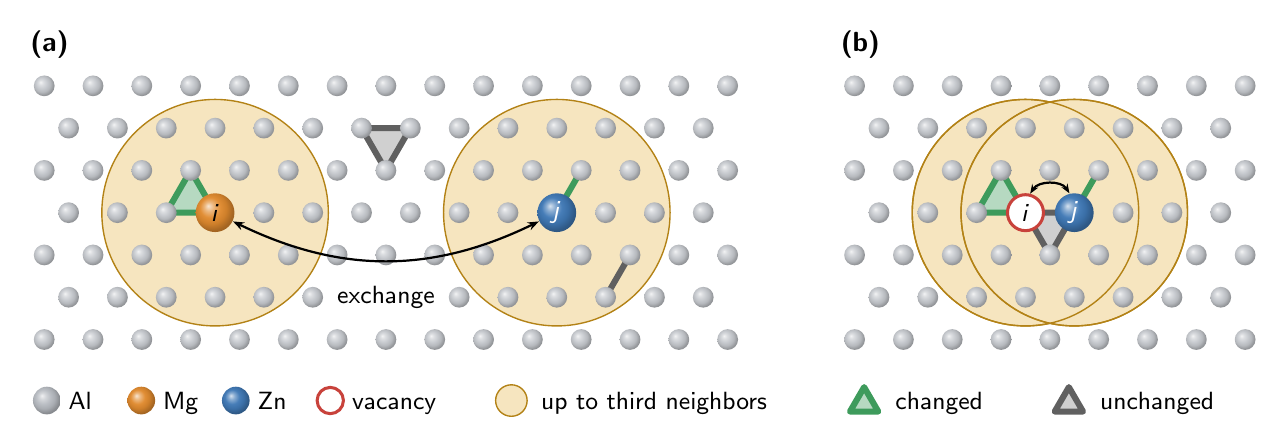
\begin{tikzpicture}[x=0.62cm, y=0.62cm,
    dot/.style={atom=cAl!80, minimum size=7.5pt},
    big/.style={minimum size=14pt, font=\small},
    reach/.style={fill=cFour!28, draw=cFour!80!black, line width=0.5pt},
    changed/.style={draw=cThree, fill=cThree!38, line width=2.2pt},
    same/.style={draw=cDark!75, fill=cDark!22, line width=2.2pt}]
  % a triangular lattice with rows at distances \h; a circle of radius 2.32 holds the first three neighbor shells (1, 1.73 and 2)
  \pgfmathsetmacro{\h}{sqrt(3)/2}
  \newcommand{\lattice}[2]{% last site of the even rows and of the odd rows
    \foreach \r in {0,2,4,6} \foreach \x in {0,...,#1} \node[dot] at (\x,\r*\h) {};
    \foreach \r in {1,3,5} \foreach \x in {0,...,#2} \node[dot] at (\x+0.5,\r*\h) {};}
  % ---------------- (a) distant sites ----------------
  \begin{scope}
    \draw[reach] (3.5,3*\h) circle (2.32) (10.5,3*\h) circle (2.32);
    \draw[changed] (3.5,3*\h) -- (2.5,3*\h) -- (3,4*\h) -- cycle;
    \draw[changed] (10.5,3*\h) -- (11,4*\h);
    \draw[same] (6.5,5*\h) -- (7.5,5*\h) -- (7,4*\h) -- cycle;
    \draw[same] (11.5,\h) -- (12,2*\h);
    \lattice{14}{13}
    \node[atom=cMg, big] (i) at (3.5,3*\h) {$i$};
    \node[atom=cZn, big, text=white] (j) at (10.5,3*\h) {$j$};
    \draw[dbl] (i) to[bend right=26] (j);
    \node[fill=white, inner xsep=1.5pt, inner ysep=2.5pt] at (7,\h) {exchange};
    \node[above lab] at (-0.35,6*\h+0.5) {\panel{a}};
  \end{scope}
  % ---------------- (b) neighboring sites ----------------
  \begin{scope}[shift={(16.6,0)}]
    \fill[reach] (3.5,3*\h) circle (2.32);
    \fill[reach] (4.5,3*\h) circle (2.32);
    \draw[reach, fill=none] (3.5,3*\h) circle (2.32) (4.5,3*\h) circle (2.32);
    \draw[changed] (3.5,3*\h) -- (2.5,3*\h) -- (3,4*\h) -- cycle;
    \draw[changed] (4.5,3*\h) -- (5,4*\h);
    \draw[same] (3.5,3*\h) -- (4.5,3*\h) -- (4,2*\h) -- cycle;
    \lattice{8}{7}
    \node[vac, big, minimum size=13pt] (i) at (3.5,3*\h) {$i$};
    \node[atom=cZn, big, text=white] (j) at (4.5,3*\h) {$j$};
    \draw[{Stealth[length=3.4pt]}-{Stealth[length=3.4pt]}, line width=0.8pt] (i.76) to[out=58, in=122, looseness=1.0] (j.104);
    \node[above lab] at (-0.35,6*\h+0.5) {\panel{b}};
  \end{scope}
  % ---------------- legend ----------------
  \begin{scope}[shift={(-0.35,-1.25)}, x=1cm, y=1cm]
    \specieslegend{0.25}{0}
    \vacancylegend{3.85}{0}
    \draw[reach] (6.15,0) circle (0.2); \node[leg] at (6.45,0) {up to third neighbors};
    \draw[changed] (10.45,-0.14) -- ++(0.36,0) -- ++(-0.18,0.31) -- cycle; \node[leg] at (10.95,0) {changed};
    \draw[same] (13.05,-0.14) -- ++(0.36,0) -- ++(-0.18,0.31) -- cycle; \node[leg] at (13.55,0) {unchanged};
  \end{scope}
\end{tikzpicture}
\end{document}
